\documentclass[a4paper,12pt]{extarticle}
\usepackage[margin=1.5cm]{geometry}
\usepackage{amsmath, amssymb}
\usepackage{array}
\usepackage{multicol}
\usepackage{helvet}
\usepackage{multirow}
\usepackage{graphicx}
\renewcommand{\baselinestretch}{2}
\renewcommand{\familydefault}{\sfdefault}

\begin{document}

    \begin{tabular}{| c | c | c | c |}
        \hline
        & MATEMÁTICAS & 16/03/2026 & calificación \\
        \hline 

        \multirow{2}{*}{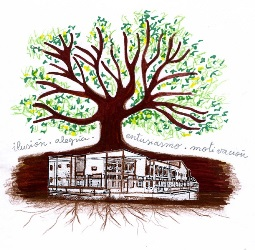
\includegraphics{../../img-Logos/iesoGalileo.jpg}} & Nombre y apellidos \hspace{120pt} & Ex. 2º ESO UD5:  & \\ 
        &&Sistemas de Ecuaciones& \\ 
        \hline
    \end{tabular}
    
    \begin{tabular}{| l | }
        \hline
        NOTAS: \\ 
            1. El examen tiene que ser limpio, ordenado y sin faltas de ortografía. \\
            
            2. El examen ha de realizarse en bolígrafo negro o azul, evitando tachones en la medida \\
            de lo posible. \\ 
            
            3. Deben aparecer todas las operaciones NO vale con indicar solo el resultado.\\
            
            4. Los problemas deben contener: Datos, planteamiento y resolución, respondiendo a lo \\
            que se pregunte, NO vale con indicar un número como solución del problema.\\

            5. Persona que se vea copiando o hablando con un compañero tiene un cero en el examen\\

            6. NO está permitido el uso de calculadoras \\
        \hline
    \end{tabular}

    \begin{enumerate}
        \item (0,5 puntos) Indica cuál de estas ecuaciones es lineal
            \begin{enumerate}
                \item $2x^3+y=5$
                \item $2xy-6=2$
                \item $2x+3y=x+y-6$
                \item $y^2-x=8$
            \end{enumerate}
        \item (0,5 puntos) Encuentra tres soluciones para la ecuación:
        \[ x - 3y =6\] $\vspace{4cm}$ 
        \item (1 punto) Expresa mediante una ecuación con dos incógnitas las siguientes afirmaciones:
            \begin{enumerate}
                \item (0.5 puntos) La suma de dos números menos su diferencia es igual a 10. $\vspace{0.5cm}$ 
                \item (0.5 puntos) La mitad del producto de dos números es 120. $\vspace{0.5cm}$ 
            \end{enumerate}
        \item (2 puntos) Resuelve el siguiente sistema
        
            $\left \{\begin{array}{rr}
                    x+2y=5 \\
                    2x+y=7
                \end{array}\right .$ $\vspace{5cm}$ 

        \item (2 puntos)epresenta el siguiente sistema e indica cuál sería la solución.
        
        $\left \{\begin{array}{rr}
                -2x+y=1 \\
                x+2y=2
            \end{array}\right .$ 


        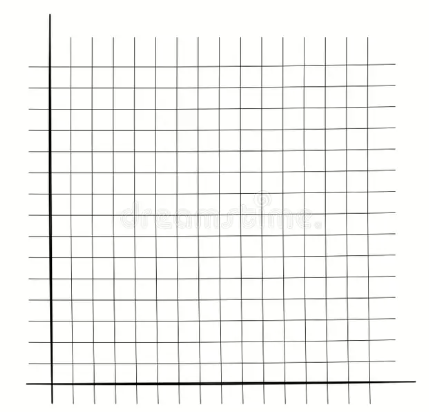
\includegraphics{img/cuadricula.png} $\vspace{7cm}$ 

        \item (2 puntos) En un patio de una escuela infantil hay triciclos y cochecitos. En total son 20 y todas las ruedas suman 67. ¿Cuántos triciclos y cuántos cochecitos hay en el patio?$\vspace{7cm}$ 
        \item (2 puntos) Mónica ha metido 15 canastas entre triples y tiros libres. Ha obtenido 43 puntos en total. ¿Cuántos triples y tiros libres (de un punto) ha anotado?$\vspace{7cm}$ 
    \end{enumerate}
\end{document}